\documentclass{beamer}
\usepackage[utf8]{inputenc}
\usepackage[T1]{fontenc}
\usepackage[slovene]{babel}
\usepackage{array}
\usepackage{booktabs} 

\newcommand{\lay}[1]{\includegraphics[width=0.40\textwidth,height=0.30\textheight,keepaspectratio]{#1}}

\usepackage{siunitx}
\sisetup{locale = SI}

\title{Reverzibilni polni seštevalniki v QCA}
\subtitle{Vrata Torresa in sod.\ proti klasičnim in logično reverzibilnim izvedbam}
\author{Denis Balant, Domen Breznik}
\institute{NPMP, skupina 19}
\date{23.~november~2026}

\begin{document}

\frame{\titlepage}

\begin{frame}
\frametitle{Motivacija za reverzibilnost}

\begin{center}
\parbox{0.8\textwidth}{\centering\vspace{0.4em}
{\LARGE $kT\ln 2 = \SI{0.0597}{\milli\electronvolt}$ pri \SI{1}{\kelvin}}\\[0.3em]
{\small najmanjša energija za izbris enega bita (Landauer, 1961)}\vspace{0.4em}}
\end{center}

\vspace{1em}
\begin{itemize}
\item Majoritetna vrata preslikajo tri vhode v en izhod, zato informacijo o
      vhodih izbrišejo.
\item Logično reverzibilna vezja QCA so večinoma zgrajena iz istih vrat in
      znotraj še vedno brišejo informacijo (npr.\ seštevalnik Ahmada in sod., 2018).
\end{itemize}
\end{frame}

\begin{frame}
\frametitle{Reverzibilna majoritetna vrata}

\begin{columns}[c]
\begin{column}{0.40\textwidth}
\centering
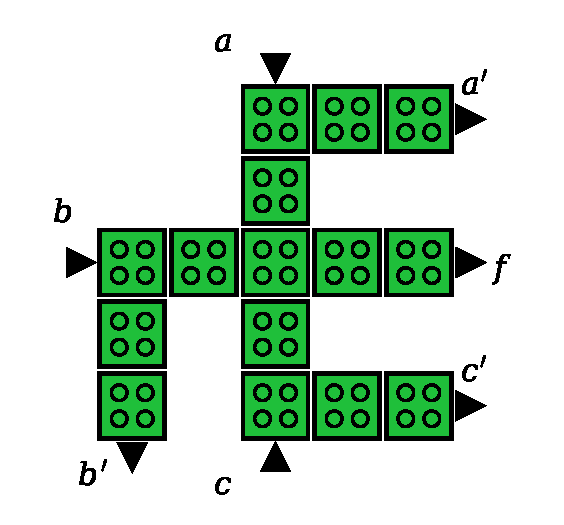
\includegraphics[width=\linewidth]{torres_vrata}\\[0.3em]
{\footnotesize Prirejeno po Torres in sod.\ (2019)}
\end{column}

\begin{column}{0.65\textwidth}
\begin{itemize}
\item Poleg izhoda $f = M(a,b,c)$ ohranijo še kopije vhodov $a'$, $b'$, $c'$.
\item Preslikava $3 \to 4$ je injektivna: vhode lahko obnovimo (neskladje z našo definicijo!).
\item Pri počasnejši uri (\SI{400}{\pico\second}) manj kot $kT\ln 2$ na operacijo.
\item Avtorji so sestavili le polovični seštevalnik.
\end{itemize}
\end{column}
\end{columns}
\end{frame}

\begin{frame}
\frametitle{Raziskovalno vprašanje}

\begin{block}{}
\centering\large
Ali polni seštevalnik iz vrat Torresa in sod.\ disipira manj kot
ireverzibilni in logično reverzibilni seštevalniki?
\end{block}

\vspace{1em}
\begin{itemize}
\item Kako je to odvisno od hitrosti ure?
\item Kakšna je cena v celicah, površini in zakasnitvi?
\end{itemize}

\end{frame}

\begin{frame}
\frametitle{Pričakovani rezultati}

\begin{itemize}
\item Pri kratki periodi ure je disipacija sorazmerna z velikostjo vezja,
      reverzibilnost ne prinese bistvene prednosti.
\item Pri počasnejši uri seštevalnik s Torresovimi vrati disipira manj od
      ostalih in pade pod $kT\ln 2$.
\item Zgolj logično reverzibilen seštevalnik disipira približno toliko kot
      ireverzibilni.
\item Cena reverzibilnosti je več celic in večja zakasnitev.
\end{itemize}

\end{frame}

\begin{frame}
\frametitle{Dve zasnovi s tremi majoritetnimi vrati}

\begin{columns}[t]
\begin{column}{0.50\textwidth}
\centering
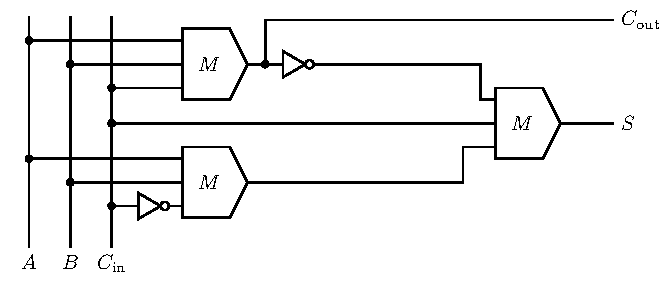
\includegraphics[width=\linewidth]{wang}\\[0.4em]
Wang in sod.\ (2003)\\[0.4em]
{\small
$S = M\bigl(C_\mathrm{in}, \overline{C_\mathrm{out}}, M(A, B, \overline{C_\mathrm{in}})\bigr)$\\[0.2em]
$C_\mathrm{out} = M(A, B, C_\mathrm{in})$
}

\end{column}

\begin{column}{0.50\textwidth}
\centering
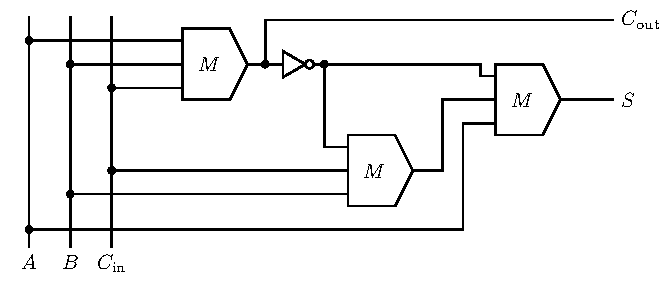
\includegraphics[width=\linewidth]{pudi}\\[0.4em]
Pudi in Sridharan (2012)\\[0.4em]
{\small $S = M\bigl(\overline{C_\mathrm{out}}, M(C_\mathrm{in}, \overline{C_\mathrm{out}}, B), A\bigr)$\\[0.2em]
$C_\mathrm{out} = M(A, B, C_\mathrm{in})$
}
\end{column}
\end{columns}

\end{frame}

\begin{frame}
\frametitle{Izvedba vezij s klasičnimi in Torresovimi majoritetnimi vrati}

\centering
\setlength{\tabcolsep}{3pt}
\begin{tabular}{>{\small}m{0.9cm} >{\centering\arraybackslash}m{0.45\textwidth} >{\centering\arraybackslash}m{0.45\textwidth}}
 & {\small Klasična vrata} & {\small Vrata Torresa in sod.} \\
Wang & \lay{wang_irr} & \lay{wang_torres} \\
Pudi & \lay{pudi_irr} & \lay{pudi_torres} \\
\end{tabular}

\end{frame}

\begin{frame}
\frametitle{Objavljeni vezji za primerjavo}

\begin{columns}[t]
\begin{column}{0.58\textwidth}
\centering

\includegraphics[width=\linewidth,height=0.5\textheight,keepaspectratio]{ahmad2018}\\[0.4em]
Ahmad in sod.\ (2018)\\
{\small navzven logično reverzibilen, 121 celic}
\end{column}

\begin{column}{0.38\textwidth}
\centering

\includegraphics[width=\linewidth,height=0.5\textheight,keepaspectratio]{seyedi}\\[0.4em]
Seyedi in J.\ N.\ (2022)\\
{\small ireverzibilen, 18 celic v treh plasteh}
\end{column}
\end{columns}

\end{frame}

\begin{frame}
\frametitle{Simulacija v QCADesigner-E}

\begin{itemize}
\item Koherenčni simulator, privzete nastavitve, $T = \SI{1}{\kelvin}$
\item Ura s periodami \SIlist{4;40;400}{\pico\second} (kako vpliva?)
\item Energija: povprečna disipacija v okolico na seštevanje (\textit{Avg\_Ebath})
\item Celic vhodnih in izhodnih vodil ne štejemo, kot Torres in sod.
\end{itemize}

\vspace{1em}
\centering
Primerjava z limito $kT\ln 2 = \SI{0.0597}{\milli\electronvolt}$ pri \SI{1}{\kelvin}

\end{frame}

\begin{frame}
\frametitle{Lastnosti implementacij}

\centering
\small
\setlength{\tabcolsep}{4pt}
\begin{tabular}{l S[table-format=3.0] S[table-format=1.3] S[table-format=1.0] S[table-format=1.2] S[table-format=1.0] S[table-format=1.2]}
\toprule
Zasnova & {Celice} & {Površina} & {Križanja} & {Zakasnitev} & {Dodatni} & {$\min|P|$} \\
        &          & {(\si{\micro\meter\squared})} & & {(cikli)} & {izhodi} & \\
\midrule
Pudi kl.  & 153 & 0.202 & 2 & 1.75 & 0 & 0.95 \\
Pudi T.   & 171 & 0.189 & 2 & 1.75 & 5 & 0.95 \\
Wang kl.  & 157 & 0.196 & 3 & 1.50 & 0 & 0.95 \\
Wang T.   & 187 & 0.196 & 3 & 1.50 & 7 & 0.95 \\
\midrule
Ahmad     & 121 & 0.143 & 0 & 1.25 & 3 & 0.95 \\
Seyedi    & 18  & 0.014 & 0\rlap{$^\ast$} & 0.50 & 0 & 0.92 \\
\bottomrule
\end{tabular}

\vspace{0.6em}
{\footnotesize $^\ast$ tri plasti brez križanj}

\vspace{1em}
Vrata Torresa: 12--20\,\% več celic, enaka zakasnitev in polarizacija
\end{frame}

\begin{frame}
\frametitle{Disipirana energija na seštevanje pri treh periodah ure}

\centering
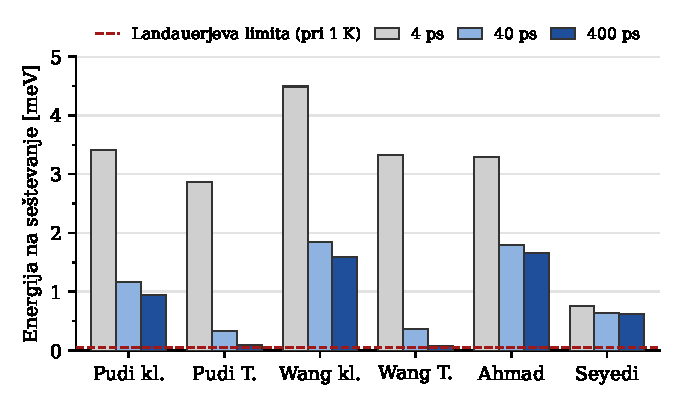
\includegraphics[width=\textwidth,height=0.72\textheight,keepaspectratio]{fig_energija}

\vspace{0.4em}
{\small Pri \SI{4}{\pico\second} disipacija sledi velikosti vezja, pri \SI{400}{\pico\second} pa vrata Torresa izstopajo.}
\end{frame}

\begin{frame}
\frametitle{Preverjanje hipotez}

\centering
\small
\renewcommand{\arraystretch}{1.3}
\begin{tabular}{l l}
\toprule
Hipoteza & Rezultat \\
\midrule
Pri hitri uri disipacija sledi velikosti vezja & delno \\
Pri počasni uri vrata Torresa disipirajo manj & drži, 10--20$\times$ manj \\
Disipacija pod $kT\ln 2$ na seštevanje & ne drži, najmanj 1,3\,$kT\ln 2$ \\
Disipacija: logično reverzibilno $\approx$ ireverzibilno & drži \\
Cena reverzibilnosti je več celic in zakasnitev & delno, 12--20\,\% več celic \\
\bottomrule
\end{tabular}

\vspace{1em}
Potrdili smo ugotovitev Torresa in sod., da mora biti perioda ure dovolj dolga.

\end{frame}

\begin{frame}
\frametitle{Omejitve}

\begin{itemize}
\item Simulacija v enem orodju pri enem naboru parametrov
\item Postavitve so ad hoc in neoptimizirane
\item Informacija prenesena na dodatne izhode: brisanje smo prenesli, ne odpravili
\item Vrata Torresa ne delujejo v obratni smeri
\end{itemize}

\end{frame}

\begin{frame}
\frametitle{Zaključek}

Vrata Torresa in sod.\ prihranijo energijo šele pri dovolj počasni uri: pri \SI{400}{\pico\second} 10--20$\times$ manj disipacije za 12--20\,\% več celic.

\vspace{1.5em}
Nadaljnje delo:
\begin{itemize}
\item kaj narediti z dodatnimi izhodi v večbitnem seštevalniku,
\item vrata, ki delujejo tudi v obratni smeri.
\end{itemize}

\end{frame}


\end{document}

